
\documentclass[12pt]{article}
\usepackage[utf8]{inputenc}
%\usepackage[latin1]{inputenc}
\usepackage[T1]{fontenc} 
\usepackage[french]{babel}
\usepackage{amsmath}
\usepackage{amssymb}
\usepackage{stmaryrd}
\usepackage{siunitx}
\usepackage{pdfpages}
\usepackage{graphicx}
\usepackage{tikz}
\usepackage{multirow}
%\usetikzlibrary{babel}
\usepackage[top = 2cm, bottom = 2cm, left = 2cm, right = 2cm]{geometry}

\newcommand{\HRule}{\rule{\linewidth}{0.4mm}} % Defines a new command for the horizontal lines, change thickness here

%%%%%%%%%%%%%%%%%%%%%%%%
\tikzset{flip flop/port labels/.initial={\tiny}}
\makeatletter
%
% better to create a family, but as an example...
\tikzset{flip flop/port labels/.initial={\tiny}}
%
% number of ports
\tikzset{ports/.initial=4}
%
% we need a counter
\newcount\tmp@a

\pgfdeclareshape{reg}{

    % you have to save the relevant parameters as \savedmacro
    \savedmacro\numports{
        \edef\numports{\pgfkeysvalueof{/tikz/ports}}%
    }
    % and \saveddimen
    \saveddimen\pinsdelta{
        % you can't use savedmacros nor savedanchors here (bummer!)
        \edef\numports{\pgfkeysvalueof{/tikz/ports}}%
        \pgfmathsetlength\pgf@x{0.22*3cm/(\numports+1)}%
    }

    % The 'minimum width' and 'minimum height' keys, not the content, determine
    % the size
    \savedanchor\northeast{%
        \pgfmathsetlength\pgf@x{3.5cm}%
        \pgfmathsetlength\pgf@y{5cm}%
        \pgf@x=0.11\pgf@x
        \pgf@y=0.15\pgf@y
    }
    % This is redundant, but makes some things easier:
    \savedanchor\southwest{%
        \pgfmathsetlength\pgf@x{3.5cm}%
        \pgfmathsetlength\pgf@y{5cm}%
        \pgf@x=-0.11\pgf@x
        \pgf@y=-0.15\pgf@y
    }
    % Inherit from rectangle
    \inheritanchorborder[from=rectangle]

    % Define same anchor a normal rectangle has
    \anchor{center}{\pgfpointorigin}
    \anchor{north}{\northeast \pgf@x=0pt}
    \anchor{east}{\northeast \pgf@y=0pt}
    \anchor{south}{\southwest \pgf@x=0pt}
    \anchor{west}{\southwest \pgf@y=0pt}
    \anchor{north east}{\northeast}
    \anchor{north west}{\northeast \pgf@x=-\pgf@x}
    \anchor{south west}{\southwest}
    \anchor{south east}{\southwest \pgf@x=-\pgf@x}
    \anchor{text}{
        \pgfpointorigin
        \advance\pgf@x by -.5\wd\pgfnodeparttextbox%
        \advance\pgf@y by -.5\ht\pgfnodeparttextbox%
        \advance\pgf@y by +.5\dp\pgfnodeparttextbox%
    }

    % Define anchors for signal ports

    \anchor{CLK}{
        \pgf@process{\northeast}%
        \pgf@x=0\pgf@x%
        \pgf@y=-1.1\pgf@y%
    }
	\anchor{C}{
		\pgf@process{\northeast}%
		\pgf@x=0\pgf@x%
		\pgf@y=-\pgf@y%
		\pgfmathsetlength\pgf@xx{1.3ex}
		\advance\pgf@y by -\pgf@xx
	}
    \anchor{D}{
        \pgf@process{\northeast}%
        \pgf@x=-1.5\pgf@x%
        \pgf@y=0\pgf@y%
    }

    \anchor{Q}{
        \pgf@process{\northeast}%
        \pgf@x=1.5\pgf@x%
        \pgf@y=0\pgf@y%
    }

    % Draw the rectangle box and the port labels
    \backgroundpath{
        % Rectangle box
        \pgfpathrectanglecorners{\southwest}{\northeast}

        % Drawing Triangle for clock input
        % upper left x
        \southwest \pgf@xa=\pgf@x \pgf@ya=\pgf@y \pgf@yb=\pgf@y
        \northeast \pgf@xb=\pgf@x
        \pgf@anchor@reg@CLK
        \pgf@xc=\pgf@x \pgf@yc=\pgf@y
        \pgfmathsetlength\pgf@x{1.3ex}
        \advance\pgf@xa by 1.5mm
        \advance\pgf@xb by -1.5mm
        \advance\pgf@yc by \pgf@x
        \pgfpathmoveto{\pgfpoint{\pgf@xa}{\pgf@ya}}
        \pgfpathlineto{\pgfpoint{\pgf@xb}{\pgf@yb}}
        \pgfpathlineto{\pgfpoint{\pgf@xc}{\pgf@yc}}
        \pgfclosepath


        \tikzset{flip flop/port labels} % Use font from this style
        \tikz@textfont



        %Drawing CLK circuit
        \pgf@anchor@reg@south
        \pgf@ya=\pgf@y
        \pgf@anchor@reg@CLK
        \pgf@xa=\pgf@x 
        \pgf@xb=\pgf@x \pgf@yb=\pgf@y
        \pgfmathsetlength\pgf@x{1.8ex}
        \advance\pgf@yb by -\pgf@x
        \pgfpathmoveto{\pgfpoint{\pgf@xa}{\pgf@ya}}
        \pgfpathlineto{\pgfpoint{\pgf@xb}{\pgf@yb}}
        %Draw clock label
        %\pgf@anchor@reg@CLK\pgftext[base,at={\pgfpoint{\pgf@x}{\pgf@y}}]{\raisebox{-2.5ex}{CLK}}

        %Drawing PC circuit
        \pgf@anchor@reg@D
        \pgf@ya=\pgf@y \pgf@yb=\pgf@y \pgf@xa=\pgf@x
        \pgf@anchor@reg@west
        \pgf@xb=\pgf@x
        %\pgfmathsetlength\pgf@x{2.7ex}
        %\advance\pgf@xb by \pgf@x
        \pgfpathmoveto{\pgfpoint{\pgf@xa}{\pgf@ya}}
        \pgfpathlineto{\pgfpoint{\pgf@xb}{\pgf@yb}}
        \pgf@anchor@reg@D\pgftext[base,at={\pgfpoint{\pgf@x+3.5ex}{\pgf@y}}]{\raisebox{-0.7ex}{D}}

        %Drawing PC' circuit
        \pgf@anchor@reg@Q
        \pgf@ya=\pgf@y \pgf@yb=\pgf@y\pgf@xa=\pgf@x
        \pgf@anchor@reg@east
        \pgf@xb=\pgf@x
        %\pgfmathsetlength\pgf@x{2.5ex}
        %\advance\pgf@xb by \pgf@x
        \pgfpathmoveto{\pgfpoint{\pgf@xa}{\pgf@ya}}
        \pgfpathlineto{\pgfpoint{\pgf@xb}{\pgf@yb}}
        \pgf@anchor@reg@Q\pgftext[base,at={\pgfpoint{\pgf@x-3.5ex}{\pgf@y}}]{\raisebox{-0.7ex}{Q}}
    }

    % create input anchors
    % this touch internal things, so beware...
    % anchors are named pgf@anchor@<name-of-the-shape>@<name of the anchors>
    \pgfutil@g@addto@macro\pgf@sh@s@reg{%
        \tmp@a=\numports\relax
        \pgfmathloop%
        \ifnum\pgfmathcounter>\tmp@a%
        \else%
        % assign the anchor "in \pgfmathcounter" to the macro \reg@port with the number as argument
        \expandafter\xdef\csname pgf@anchor@reg@in \pgfmathcounter\endcsname{%
            \noexpand\reg@port{\pgfmathcounter}% defined below
        }%
        % \typeout{YAY\space\pgfmathcounter}
        \repeatpgfmathloop%
    }

}
%
\def\reg@port#1{%
    % this macro has the function to return the position of the anchor
    % it must use only \savedanchors and \savedmacros
    % the parameter is the number of the anchor (see above)
    \northeast
    \pgf@x=-\pgf@x
    \pgf@ya=\pgf@y
    \pgfmathsetlength{\pgf@y}{\pgf@ya-(#1+0.5)*\pinsdelta}%
}
\makeatother

%\newcommand{\reg2}[1]{%
%\begin{tikzpicture}
%  \draw (0,0) rectangle (1,1.5);
%  \draw (0.3,0) -- (0.5,0.2) -- (0.7,0);
%  \draw (0.5,1) node{D Q};
%  \coordinate (0,1) coordinate (D);
%  \coordinate (1,1) coordinate(Q);
%\end{tikzpicture}}


\title{Synthesis ELEC2570}
\author{Louis Devillez}
\date{\today}

\begin{document}

\maketitle

\tableofcontents
\section{Design Flow}
\begin{enumerate}
  \item Concept
  \item High-level design: Arch. description and embedded program
  \item RTL coding
  \item Behavorial simulation and verification: HDL code
  \item Logic synthesis: Structural netlist
  \item Structural simulation: Masks layout
  \item Place and route: Physical netlist
  \item Physical simulation and sign-off: Tape-out
  \item Fabrication: Silicon wafer (silicon die for 1 unit on the wafer)
  \item Dicing and Assembly (packaging and wire bonding): Chip
  \item Testing and sorting: product
\end{enumerate}

\textbf{Fab-less company}: from Concept to Signoff

\textbf{Pure-play foundry:} from Signoff to Testing

\textbf{NRE:} Non-recursive Engineering (cost)
      
\section{Module A: From C code to embedded execution}
\subsection{PPA}
The PPA is a good factor to evaluate a digital chip
\begin{itemize}
  \item Speed \textbf{P}erformance in GHz:
    \subitem \(f_{clk} \rightarrow\) CPI (not enough)
    \subitem MIPS (cpu) or GOPS/GFLOPS
  \item \textbf{P}ower consupmiton in mW:
    \subitem \(P \propto f_{_{clk}} \rightarrow\) Needs to be normalized
      \subitem mW/MHz, GOPS/W, pJ/inst, \(\mu\)J/task
    \item Fabrication costs \(\propto\) 1/ Silicon \textbf{A}rea
\end{itemize}

\textbf{CPI:} Clock per instruction.

\textbf{GOPS:} Giga operation per second.

\textbf{GFLOPS:} Giga floating operation per second.



\subsection{Business model map}
\begin{itemize}
  \item IP vendors: produce hardware and software intellectual property
  \item Semiconductor vendors: produce digital design
  \item EDA and foundries: implement IC design on silicon
  \item OEMs and ODMs
  \item Software developers
  \item Operators
  \item Retailers
  \item Consumer
\end{itemize}
\bigbreak
\textbf{IP:} Intellectual property.

\textbf{EDA:} Electronic design automation

\textbf{OEMs:} Original equipment manufacturer

\textbf{ODMs:} Original Design manufacturer


% TODO add relations ?

\subsection{MCU}
Microcontroller are often used in embedded applications. The embeds various functions (IO,I2C, memory, ADC,DAC, Timer, Power management Unit, CPU). Low cost (high production volume).
\bigbreak
Two main CPU: \textit{ARM Cortex-M} and \textit{RISC-V}. Cortex-M0 are predictable (in-order execution, built-in interrupt controller), portable (predetermined memory space)
\bigbreak
\textbf{Thumb instruction set:} 16 bits instructions (limit code size). Subset of ARM instruction. Only the branch is conditional.
\bigbreak
\subsubsection{Processor core}
\textbf{Harvard architecture:} 2 bus - 1 for data and 1 for instruction.

\textbf{Von Neumann architecture:} 1 bus for data and instruction.
\bigbreak
16x32-bit registers
\begin{itemize}
  \item R0 - R12: general use register
  \item R13: Main stack pointer/Process stack pointer
  \item R14: Link register
  \item R15: Program counter
\end{itemize}

Only 16 registers to stay low poer and have compact instructions.
\bigbreak
\textbf{Fast 32-bit multiplier}: single cycle (in SW, 32 instructions) (optional)

\textbf{Floating point hardware}: (optional)


\subsubsection{Interrupt}
\textbf{NVIC:} Nested vector interrupt control

\textbf{WIC:} Wake-up interrupt controller

\textbf{NMI:} Non-maskable interrupt



\subsection{AHB}
\textbf{AMBA:} Advanced Microcontroller Bus Architecture

\textbf{AHB:} Advanced High-performance Bus, high bandwidth (pipeline, burst transfers, single-cycle master handover)

\textbf{APB:} Advanced Peripheral bus - low bandwith, low complexity

\textbf{AHB-Lite:} Subset of AHB. High performance bus:
\begin{itemize}
  \item Two-cycle transfer: address phase, then data phase
  \item Wide data bus configuration (32-bit to 102B-bit data)
  \item Burst transfers and wait states
  \item single-clock dege operation
  \item MUX operation
\end{itemize}


\subsection{RAM and memory}
The RAM contains:

\textbf{Data:} static and global variables

\textbf{Stack:} temporary variable and parameters of functions call

\textbf{Heap:} dynamically allocated variables

The stack and heap grow in opposite directions.

The cortex-M0 can generate byte, half-ward, and word transfers

\subsection{Architectural design}

\textbf{RTL:} Register transfer level

\textbf{High-level synthesis:} Synthesize RTL code from C/SystemC/Matlab. Improved productivity but PPA still lagging far behind manuel coding.
\bigbreak

Need SoC verification: First-time success is paramount and verefication is key (sooner the error is detected, the quicker a fix is implemented).

\textbf{Verification:} act of reviewing, inspecting and testing a design ir order to establish that it meet the specifications (functional and performance).

\subsubsection{Dynamic verification}
\textbf{Dynamic verification:} Simulate the design with a given set of stimuli to check thats its state and outputs are correct (performed at all design stages).

The number of states grow too fast (\(\log^2\)) and worst with CPU (test all SW). A possibility is to emulate the design on a fpga (SW developement before SoC production) but:
\begin{itemize}
  \item Require time and expertise
  \item is also subject to human errors
  \item Dose not capture layout effects
\end{itemize}

A test bench is used to provide and collect data. Need also a clock and reset signal. (Testbench should be written by a different person than the designer). Waveform inspection or sequential generation of input stimuli is not scalable. Complex DSP need high-level model to compare the outputs.


\textbf{Assertions based verification:} a statement that a certain property must be true, which falgs an error if not. It is possible to check block internal state. Can be specified by designer of verificatino teams. Widely adopted by the industry when there is a lot of IP blocks.

\bigbreak
ABV can be used for measuring test coverage. The reach a coverage of 100\% we need manual testbench improvement with new mode of operations, function, range of input stimuli. 


To cost of verification increase with the miniaturisation.

\textbf{Metric-driven verification:} use coverage-directed automatic random stimuli generation to exercise all parts of the design. Universal Verification Methodology (UVM) is a standardized metric-driven methodoly for RTL digital design with a focus on IP re-use.
\subsubsection{Formal verification}
\textbf{Formal verification:} Use of mathematical methods to prove that a design meets its specification. It is defined by
\begin{itemize}
  \item Mathematical framework
  \item Verification technique
\end{itemize}

\textbf{Logic equivalence checking:} Prove the logic equivalence between golden RTL and varisous RTL during the whole design.
\begin{itemize}
  \item Performed by a dedicated tool (e.g. Cadence Conformal)
  \item Works on both combinatorial and sequential digital circuits
  \item Complicated by low-power features
\end{itemize}


\subsubsection{Static verification}
\textbf{Static verification: } Check that several constraints are met in the design.

\section{Module B: From platfrom HDL to gate-level netlist}

\subsection{Principle}

\textbf{HDL:} Hardware description language

\textbf{Logic synthesis:} Conversion from HDL description to a gate-level netlist
\begin{itemize}
  \item HDL: Descripton of the design
  \item Constraints on the design (.sdc)
    \subitem PPA design intent constraints (e.g. timing)
    \subitem Boundary and operating conditions
  \item Target technology and libraries (.lib/.db)
  \item Output: Verilog structural netlist and Constrain file (.sdc)
    \item Tool: Synopsys Design Vision / Design compiler | Cadence RTL compiler
\end{itemize}

Steps:
\begin{enumerate}
  \item Analysis + elaboration: converts HDL to generic logic netlist
  \item Mapping: convert generic netlist into standard cells from the core library
  \item Optimization: optimizes the netlist to meet the PPA design constraints (iterative process)
  \item Lint: Netlist sanity check to make sure the RTL/netlist is valid
\end{enumerate}



\subsection{Design constraints}
\begin{itemize}
  \item Design \textbf{intent} constraints: From the designer (e.g. PPA) \(\Rightarrow\) .sdc
  \item Design \textbf{rule} constraints: from the foundra or library provider (e.g. thold) \(\rightarrow\) .db/.lib
\end{itemize}

\(\Rightarrow\) We meet first the design rule constraints to have a functionnal circuit and then the design intent constraints.


Performance trade-offs: we have a Pareto curve of optimum solutions between energy and Delay.


\subsection{Timing closure}
\textbf{Setup timing constraint:}
\[
T_{cycle} > T_{clk2Q} + T_{setup} + T_{hold}
\]

\textbf{Slack:} Difference between the timing of the capture path and of the launch path.

\textbf{STA:} Static timing analysis - method for computed the expected timing behavior of a synchronous logic circuit without simulation.


\begin{figure}[!ht]
  \centering
  \begin{tikzpicture}
   \node [draw,reg] (reg1) at (0,0) {};
   \node [draw,reg] (reg2) at (4,0) {};
   \draw (reg2.C) -- (reg1.C) -- ++ (-1.5,0);
   \draw (reg1.Q) -- (reg2.D) node[midway] (mid){};
   \node[rectangle,draw,fill=white] at (mid){CL};
   \draw [red,-latex] (-1,-0.9) -| (-0.2,0.5) -- ++ (3.8,0) node[above,midway]{Launch path};
   \draw [red,-latex] (-1, - 1.1) -| (4.2,-0.8) node[midway,right]{Capture path};
  \end{tikzpicture}
  \caption{Timing constraints}
  \label{Tikz:}
  \end{figure}

  \textbf{Timing exceptions:} Everything whose timing constraint is not defined by \(T_{cycle} > T_{C2Q} + T_{delay} + T_{setup}\) (e.g. asynchronous I/O, extremely relaxed timing constraint).


  \subsubsection{Timing closure}
  To achieve the timing closure
  \begin{itemize}
    \item Net list optimisation (simplify by moving gates)
  \item Gate mapping optimization (replace a groupe of gate by a gate).
  \item Pin swapping (invert A and B of gate to go through less transistors)
  \item Driving strength incerease
  \item Buffering centralized or distributed
  \item Pipelining (up to \(T_{setup} / T_{C2Q}\))
  \item Automatic architecture optimizations (e.g. choice the right adder to reach target PPA).
  \item Register retiming (moving register to break differently the path but can increase area and power if the number of register increase).
  \item Technology optimization (L8 and L9)
  \end{itemize}
  \subsection{Standard-cell}
  
  Type of cells:
  \begin{itemize}
  \item Combinational cells: INV, NAND, NOR, AND, OR, XOR, MUX
  \item Sequential cells: DFFQ, LATQ
  \item Implementation cells: buffers, logic0, logic1
  \end{itemize}

  Cells are available in various driving strengths (Driving capacity).
\bigbreak
Operating constraints (\textbf{PVT} corner)
\begin{itemize}
  \item \textbf{Process}: slow - typical - fast. Trade off with leakage current
  \item \textbf{Voltage:} trade off speed - power consumption
  \item \textbf{Temperature:} trade off speed - leakage current
\end{itemize}
Strategies: Typical conditions (design evaluation) or worst-cas conditions (design sign-off).

\subsection{Robust HDL coding}
\label{Robust-HDL-coding}
Non-synthesizable statements:
\begin{itemize}
  \item Initial statements (not physical) \(\Rightarrow\) restable register
  \item Delay statements \(\Rightarrow\) constraints in the .sdc OR delay the signal by clock cycles
\end{itemize}

Undesired logic:
\begin{itemize}
  \item Unwanted latch \(\Rightarrow\) add default case in \textit{if/case} statements
  \item Combinatorial feedback loops \(\Rightarrow\) break the loop with register
\end{itemize}


\subsection{Clock design}
Multiple clocks can be
\begin{itemize}
  \item Synchronous
  \item Logically exclusive 
  \item Asynchronous
\end{itemize}
\bigbreak
\begin{itemize}
  \item Must be clean (no glitch)
  \item Generated by a crystal oscillator or a PLL
  \item \textit{create\_clock} constraint in the .sdc defines how the timing analysis will be run.
\end{itemize}
\bigbreak
A multiple clock can be generated from a PLL and a clock division with a CLK gen (clock generated on chip). We need a synchronization FF at output of divided-clock to kills glitches. The C2Q delay induces a skew and there is a timing violation \(\Rightarrow\) annotate a zero delay for structural simulation.
\bigbreak
Clock inversion, Glitch reduction and clock selection must be used with strong care (may require specific constraints).
\bigbreak
If we want a selection between exclusive clock we need a glitch-free clock MUX.

\begin{figure}[!ht]
  \centering
  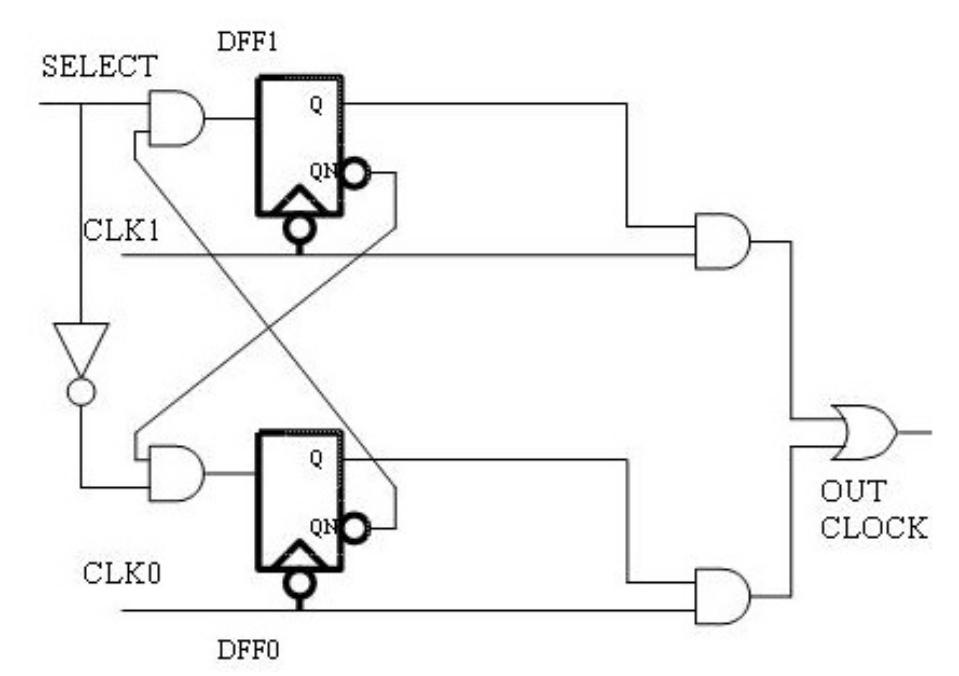
\includegraphics[width=0.45\textwidth]{Images/glitch_free_mux.png}
  \caption{Glitch-free clock MUX}
  \label{glitch-free MUX}
\end{figure}


\textbf{Metastability:} Time window \(T_W\) where setup/hold is violated. Two flip-flops in series form a double-latech barrier and improve the MTBF (Need to specify to the tool te be tolerant on \_meta nodes

\textbf{MBTF:} Mean-time between Failure \( \cfrac{e^{S/\tau}}{T_WF_CF_D}\)
\begin{itemize}
  \item \(F_C\): synchronizing clock frequency
  \item \(F_D\): data changing frequency
\item \(T_W\): probability to enter Metastability
\end{itemize}


\subsection{Reset design}
\begin{itemize}
  \item Synchronous reset: more resistant to glitches
  \item Asynchornous reset: easier design
  \item Massive reset: high fanout and bit capacity to drive
  \item to prevent timing violations with an external reset, the reset input shold be synchronized
\end{itemize}

\subsection{Logic paths}
\begin{itemize}
  \item IN2REG
  \item REG2REG
  \item REG2OUT
  \item IN2OUT
\end{itemize}
IN2OUT are very rare and a well-balanced design should have REG2REG critical paths

\bigbreak
Boundary conditions on input/output ports impact the timing and power of the design (slew rate and capacitance). To resolve IO setup constrains we can forward the clock (have the same delay between capture and lauch path).


\subsection{Power}
Average power
\begin{align}
P_{avg} = \frac{1}{T} \int_0^T i_{dd}(t) V_{dd}dt = P_{dyn}(f_{clk}) + P_{stat}
\end{align}

Switchig power (charging a node)
\begin{align}
 P_{SW} = C_L V^2_{dd} f_{clk} \alpha_f
\end{align}

Short-circuit(during input transition when both transistors are ON)
\begin{align}
  P_{SC} = C_L V^2_{dd} f_{clk} \alpha_f \beta_{SC} = P_{SW} \beta_{SC} 
\end{align}

Leakage power
\begin{align}
  P_{Leak} &= V_{dd} * W/L *\mu * C_{DEP*} U_{th}^2* 10^{(Vgs-Vt)/S *} (1 -e ^{-Vds/Uth})\\
           &= V_{dd} \beta_{sub} * 10^{(Vgs-Vt)/S *} (1 -e ^{-Vds/Uth})
\end{align}

To reduce \(I_{leak}\) we can change the \(V_t\) %TODO see later
\bigbreak

\begin{itemize}
  \item \(\alpha_f\) activity factor
  \item \(\beta_{SC}\) short circuit factor
\end{itemize}

\bigbreak

The internal power is the sum of the switching power and the short-circuit power.

The switching activity need to be annotated to have accurate power reports (.saif)
\bigbreak
\(P_{SW}\) and \(P_{leak}\) have opposite trends \(\Rightarrow\) MEP around 0.3 - 0.4V. We can reduce \(f_{clk}\) and \(V_{dd}\)  to reduce the \(P_{idle}\) (reduce by \(V_{dd}^2\)). But it is limited by memories.
\begin{itemize}
  \item Reducing \(V_{dd}\) reduce the power but increase the delay
  \item Reducing \(f_{clk}\) reduce the power but increase the delay
\end{itemize}

\textbf{MEP:} Minimum energy point
\bigbreak
\textbf{Clock gating:} Disabled register at certain clock cycles to save power (\(\alpha_F\)). The best implementation is with a Latch and a AND gate. It can be used to
\begin{itemize}
  \item Implement sleep mode and wake up with IRQ
  \item Disable unused HW acc/memories or Peripheral
\end{itemize}

\textbf{Operand isolation:} save switching power in unused combinatorial blocks can be done with AND gates or latches (manual or automatically) (\(\alpha_f\)).

\textbf{Power gating:} Disable a circuit when not used (power shut-off). But challenges: states retention, output isolation, wake-up time, wake-up rush current.


\subsection{Memories}

\begin{center}
  \begin{tabular}{|c|c|c|c|}
    \hline
    \multicolumn{2}{|c|}{Volatile}&\multicolumn{2}{c|}{Non-Volatile}\\
    \hline
    Static&Dynamic&Read only&Electricaly programmable\\
    \hline
    \hline
    SRAM macro& \textcolor{red}{DRAM macro (trench capacitor)}&ROM macro& \textcolor{red}{Flash}\\
    \hline
  \textcolor{blue}{RAM synthesized}&DRAM macro with gain cell&OTP (eFuse)&\textcolor{red}{Emerging memories}\\
    \hline
&&\textcolor{blue}{Rom synthesized}&\\
    \hline
  \end{tabular}
\end{center}
\begin{itemize}
  \item \textcolor{blue}{Standard cells}
  \item \textcolor{red}{Standalone}
  \item Can be embedded
\end{itemize}

\subsubsection{SRAM}
\begin{itemize}
  \item Write: charge bitline to the value to write
  \item Read: pre-charge bitline to Vdd/2
  \item We need stability for read and write: SNM (mV)
\end{itemize}

\textbf{SNM:} Static noise margin


Synthesized RAMs can be done with registers (for small size < 1kB). The best implementation is to register the input address and not the output (to prevent power loss due to glitches).
\bigbreak
The bigger mux will reduce the RAT but increase the power and the area.

\textbf{RAT:} Read access time





\section{Module C: From gate-level netlist to physical layout}


\subsection{Physical implementation}
\textbf{Step 1:} The floorplanning
\begin{itemize}
  \item the core size (dimension or the aspect ratio)
  \item the core to boundary distance.
  \item Core row utilisation
    \subitem High utilization (lower area and possible shorter routing (lower delay - low C)
    \subitem Low utilization (Routing less complicated, use space to do timing optimization, less heat/area)
  \item Row Organization: orientation and spacing
\end{itemize}

\textbf{Step 2:} Placement of the hard macros

\textbf{Step 3:} Placement of the well taps

\textbf{Step 4:} Power rail (width and position \(\rightarrow\) care to IR drop)

\textbf{Step 5:} Clock tree
\begin{itemize}
  \item short path are most prone to hold time violations
  \item Hold time violation cannot be fixed with a reduction of clock frequency
  \item Skew is temporal due to
    \subitem Clock source
    \subitem ambient and circuit noise
    \subitem Supply/ground bouncne
\end{itemize}
The clock tree improves skew and transition but introduce a delay. It degrade
\begin{itemize}
  \item REG2OUT setup closure
  \item IN2REG hold closure
\end{itemize}

\textbf{Step 6:} Routing
\begin{enumerate}
  \item Power nets
  \item Clock nets
  \item Signal nets (timing-driven)
\end{enumerate}
We use buffer and repeater to lower the capacitance to drive (lower \(\tau\)).

Crosstalk and Signal Integrity (SI) \(\Rightarrow\) Lower the cap



% TODO replace this
Need decap cells to reduce load to drive 

\subsection{Timing optimization}
\begin{itemize}
  \item Add/delete buffers
  \item Resize cells
  \item Restructure the netlist
  \item Remap logic
  \item Swap pins
  \item Move instances
\end{itemize}

\subsection{Packaging}
\begin{itemize}
  \item Package parsitics
  \item Wirebond inductance
\end{itemize}
ground/supply bounce at rising edge of the clock (flip-flop toggle) or whene output pad is changing (large C and large transistor). To prevent that
\begin{itemize}
  \item Parallel connection (reduce parasitic inductance), Half IO \(\rightarrow\) power pads
  \item Ground plane
\end{itemize}


\subsection{Technology scaling}

\subsubsection{5V world and happy scaling}
\textbf{Moore's law:} The number of transistor per chip doubles every 1.5-2 years

\textbf{Transistor sclaling:} Dividing \(T_{ox}\ L\ W\) by \(\alpha\)

\textbf{Interconnect:} Connection between different metal layer %TODO replace it correctly and verify it

\textbf{Interconnect scaling:} Dividing \(H_{met}\ H_{met} \ \) Pitch by \(\alpha\)

\begin{table}[!ht]
  \centering
  \begin{tabular}{|l|c|c|}
    \hline
    &Constant&Constant\\
    &Voltage&field\\
    \hline
    \hline
    Dimensions: \(W,\ L,\ T_{ox}\)& \(1/\alpha\) & \(1/\alpha\)\\
    \hline
    Voltages: \(V_{dd},\ V_t\)&1 & \(1/\alpha\)\\
    \hline
    Current par device: \(I_{on}\)&\(\alpha\) & \(1/\alpha\)\\
    \hline
    Capacitance per device: \(C_{gg}\)& \(1/\alpha\) & \(1/\alpha\)\\
    \hline
    Area&\(1/\alpha^2\) & \(1/\alpha^2\)\\
    \hline
    Delay, \(1/f_{clk}\)& \(1/\alpha^2 \) & \(1/\alpha\)\\
    \hline
    Energy per operation& \(1/\alpha\) & \(1/\alpha^3\)\\
    \hline
    Power density&\(\alpha^3\) & 1\\
    \hline
  \end{tabular}
  \caption{Transistors scaling}
  \label{Transitors-scaling}
\end{table}

Limit to constant-voltage scaling: 5V and power
\begin{itemize}
  \item Area overhead and speed penalty
  \item High power density
  \item Total power: battery lifetime concern
\end{itemize}
\bigbreak

\subsubsection{Interconnect limitation}
Limit to constant field scaling: the resistance of interconnect per length unit increases. Reduce the interconnect delay:
\begin{itemize}
  \item New inteconnect (technology)
    \subitem Change material (lower resistance)
    \subitem Change dieletric (void)
  \item New technique (Design)
    \subitem Keep high metal level for global interconnect and not scaled
    \subitem Extensive use of repeater (buffering)
\end{itemize}

\subsubsection{Leakage limitation}
When the gate length becomes too small, the leakage power dominate. To limit the static power dissipation:
\begin{itemize}
  \item Multi \(V_t\) techniques (Design) but high complexity
  \subitem Use low \(V_t\) on critical path
  \subitem Use high \(V_t\) on non-critical path (leakage reduction)
  \item Stop \(V_t\) scaling (Technology) but low speed
    \subitem Limitation \(V_t\) and \(V_{dd}\) (Velocity saturationd and mobility reduction)
    \subitem Strained-Silicon has Enhanced Mobility
\end{itemize}

\subsubsection{Gate leakage current}
The gate leakage exponentially increases with \(T_{ox}\) scaling. Short-channel effects
  \begin{itemize}
  \item Degradation of the slope,
  \item Shift of \(V_t\) (roll-off)
  \item S-D leakage current
  \end{itemize}

  \(\Rightarrow\) Process diversifacation
  \begin{itemize}
    \item Low standby power (LSTP) CMOS
    \item Low operation power (LOP) CMOS
    \item High performance (HP) CMOS
  \end{itemize}


  \(\Rightarrow\) Increase \(C_{ox}\) to limit short-channel effects \(\Rightarrow\) Change oxide material


\subsubsection{Variability and scalability}
\textbf{Speed binning:} Regroup IC by Normalized leakage and frequency (due to variability - Random dopant fluctuations \textbf{RDF}).

variability on \(V_t\) limit maximum speed and increase total leakage on large chip. It also reduce the SNM for SRAM (failures). To mitigate the variability:
\begin{itemize}
  \item New devices (technology)
    \subitem Finfet: 3D CMOS - Pricer wafer but simpler process (No significant increase)
    \subitem Full-depleted (FD) SOI: thin undoped channel (no RDF) in a buried oxide
  \item New techniques (Design)
\end{itemize}


\subsubsection{Lithography}
Since 180 nm generation, we use sub wavelength lithography
\begin{itemize}
  \item Rounding effects
  \subitem Gate length variation induces high leakage
  \subitem Higher capacitance
  \subitem Short circuit
\item Line edge roughness (\textbf{LER})
  \subitem Varialbe line resistance/capacitance
  \subitem Further \(V_t\) fluctuations
\end{itemize}

Solutions
\begin{itemize}
 \item Optical proximity correction (OPC) -> interference
 \item Resolution enhancement techniques (\textbf{RETs})
      \subitem From 45/40nm: highe numerical aperture and phase shift masks
      \subitem From 32/28nm: Immersion lithography
      \subitem From 22 nm: multiple patterning
      \subitem From 5 nm: Extreme Ultra-Violet (\textbf{EUV}) with 13nm wavelength
\end{itemize}
\(\Rightarrow\) Wafer cost is exploding


\section{Module D: HW/SW co-design}
\subsection{Hardware accelerator}
\subsubsection{General-purpose processor}
\begin{itemize}
  \item Control-oriented applications
  \item Optimized for
    \subitem Conditional branching
    \subitem Flexible data moves (block, words,GPIO,\dots)
  \item Performance metric: MIPS
  \item Instruction set architecture (\textbf{ISA}): RISC vs CISC
  \item Instruction execution: in-order vs out-of-order
  \item Memory architecture: Harvard vs Von Neumann
  \item Gpp clock speed increase due to optimizations (pipeline)
  \item Energy per instruction improved but not dramatically
\end{itemize}


\subsubsection{DSP cores}
\begin{itemize}
  \item For signal (1D) or image (2D)
  \item Optimized for
    \subitem arithmetic functions
    \subitem regular memory accesses
  \item Performance metric: GOPS
\end{itemize}

\lstinputlisting{code/DSP-pseudocode.s}

\begin{table}[!ht]
  \centering
  \begin{tabular}{|l|c|c|c|}
    \hline
    Architecture&\#cycles& \#PMEM accesses& \#DMEM accesses\\
    \hline \hline
    Von Neumann & 8N& 6N& 2N\\
    \hline
    MAC instruction& 7N&5N&2N\\
    \hline
    Harvard/Thumb ISA& 5N&5N&2N\\
    \hline
    Hardware loop& 3N& / &2N\\
    \hline
    C(i) \(\rightarrow\) PMEM& 2N& N& N\\
    \hline
    Dual mac/3bus& 2N/2& N/2& 2N/2\\
    \hline
    Delay reg& N&N/2&N/2\\
    \hline
  \end{tabular}
  \caption{Effect of DSP features (FIR loop)}
  \label{table:dsp}
\end{table}

\textbf{MAC}: Multiply accumulate, fusion of a multiplication and a addition (\(R_3 = R_3 + R_1 * R_2\))


\textbf{Hardware looping:} improve the repetition of insructions sequentially on large data blocks (vectors/arrays) by getting rid of control instructions. It requires logic resources:
\begin{itemize}
  \item Loop counter
  \item Instruction loop buffer
  \item Hardware data address generation
\end{itemize}

\textbf{Triple data bus:} Fetch data for 2 mac at once

\textbf{Delay Register:} add a delay block between the input of the two mac


\bigbreak
Key ideas:
\begin{itemize}
  \item Datapath / ALU with rich snigle-cycle arithmetic operation (MAC \dots)
  \item Memory based architecture with single-cycle multiple data accesses
  \item Specific addressing modes for loops
  \item Reduced control overhead for loops (instruction decoding, jump instructions
\end{itemize}

\textbf{SIMD:} Single-Instruction Multiple-Data is a technique of performing the same operation on multiple pieces of data simultaneously (GPUs)

\textbf{GPU:} Graphic processing units - massively parallel processor to maximize performance for graphirc workload charcterized by many fragments

\textbf{Superscalar:} a CPU implementing a form parallelism called instruction-level parallelism (\textbf{ILP}). It execute more than one instruction during a clock cycle (instruction dispatch done at execution).

\textbf{VLIW}: Very-long instruction word is a packing of single word of instruction (instruction dispatch done at compilation).

\textbf{MPSoCs:} Multi-processors Socs - When higher fully parallel performance are required


\subsubsection{Hardware accelerators}

HW accelerators are highly specialized to the functions which allows reaching very high energy/performance efficiency. The drawback is the lack of flexibility: in a generic DPS we need numerous HW accelerators (avantage on dark Silicon issues).

\textbf{Dark Silicon:} We cannot activate all transistors at once on a chip some need to stay off.
\bigbreak
Typical application
\begin{itemize}
  \item Generic: digital filters, min/max search
  \item Signal analysis: FFT
  \item Communications: convolutional encoding, error correcting codes
  \item Crypto functions: encryption/decryption, hash function
  \item Audio applications: compressions codecs
  \item Video applications: compressions codecs, image enhancement
  \item Sensor applications: Bloom filter, classifier with ML (SVM)
\end{itemize}

\subsubsection{MPSoc architectures}
Instruction fetch and datpath control has high energy cost. Memory access have also a higher energy cost. Data locality is key to have energy-efficient computing.



Single-core memory organization
\begin{itemize}
  \item Register file (2 read port + 1 write port)
    \subitem Two bottlenecks
    \subitem Separate L1 cache
    \subitem Single-bus L2 main memory
  \item The bypass bottleneck
    \subitem Bypass circuit for pipeline execution stage to get rid of stall
    \subitem Tag comparison on register index
    \subitem PPA hungry in long pipeliens
  \item The register file (\textbf{RF}) bottleneck
    \subitem VLIW share a common register file bypass network
    \subitem RF require 2N read port and N write port (not an SRAM)
    \subitem In practice, 5 issues in parallel is the maximum
\end{itemize}

\bigbreak
Interconnect fabrics
\begin{itemize}
  \item I/O-based transfers
    \subitem Specific routing network connect the I/Os of several cores together
    \subitem Low latency and power
    \subitem Lack of flexibility
    \subitem Difficult synchronization
  \item FIFO-based transfers
    \subitem Fifo as buffer between cores
    \subitem Allow asynchronicity betweeen PEs with 2 independent clocks
    \subitem Lack of flexibility
  \item Memory-based transfer
    \subitem Easier programming
    \subitem Requires cache coherency management
    \subitem Higher latency and power
  \item DMA-based transfers
    \subitem DMA allow offload the PEs of their block memory transfers
    \subitem PE sends a requets to the DMA and goes back to work/sleep
    \subitem Several bus architecture can support DMA transfer (bus becomes a bottleneck when many PEs are interconnected).
  \item Network on chipts (\textbf{NoCs})
    \subitem Ultimate solution for many-core GALS architecture
    \subitem Each PE/SE is a node connectd by a router (including FIFO)
    \subitem PE/SEs can have independent embedded \(V_{dd}\) and clock generator
    \subitem Can re-use all the techniques from the off-chip communication networks (TDMA, CDMA\dots)
\end{itemize}



\subsection{Anthroposcene}

\textbf{Absolute resource footprint:} KPI unit x Intensity

\textbf{KPI:} Key performance indicator

\begin{align}
  CO_2e = Pop * \frac{A}{Pop} * \frac{E}{A} * \frac{CO_2e}{E}
\end{align}

\bigbreak
Observations
\begin{itemize}
  \item The followup of efficiency-improvement laws did not lead carbon footprint reduction
  \item Affluence increases mor than the efficiency
\end{itemize}

\bigbreak
Hypothesis
\begin{enumerate}
  \item The impossibility of green growth
    \subitem Increasing KPI is the way to generate economic growth
    \subitem Decoupling between economic growth and energy footprint
  \item Escalating NRE costs
    \subitem All KPI are bounded by a physical limit
    \subitem Getting closer to the limit requires increasing innovation investetments (NREs)
    \subitem Return on investment requires increasing the affluence
    \subitem Companies compete to attrack capitals by promising growth of the stock value (speculative capitalism instead of accumulative)
  \item ICT innovation pitfalls
    \subitem KPI innovation (e.g. 5G)
    \subitem Buzzword-driven innovation (ML for energy-efficiency optimization).
\end{enumerate}


Consequences
\begin{itemize}
  \item Creation of artificial needs
  \subitem High emission form onlive video
  \item Obsolescence generation
\end{itemize}



\subsection{Ecological transition in ICT}
\begin{enumerate}
  \item Focus innovation on human needs
    \subitem Don't create needs
    \subitem Needs human interaction with the rest of the world
  \item Replace KPI drive by reduction in carbon / resource footprint
  \item Limit rebound effects
    \subitem How will this innovation be used
    \subitem Can we prevent abusive/unlimited use 
    \subitem Needs for multidisciplinarity
\end{enumerate}






\section{Homework}
\subsection{A1}

We can find those name at output of the compiler:
\begin{itemize}
  \item Code: pure code
  \item RO: Read Only (eg. image input)
  \item RW: Read and write (data)
  \item ZI: zero init data (stack and heap)
\end{itemize}
\bigbreak
The iROM is a non volatile memory and iRAM is a volatile memory (for stack + heap + \dots). We need ram, because flash memory (ROM) has a limited number of writing and RAM is also low power.

The heap is built in a ascending way and the stack is built in a descending way. If we go out of boundary we will have corruption (for example with the 64*128 image)

\bigbreak
The main is not the first thing executed in a program. We need initialization whchi will perpare the system to run the main. It can be observed after a reset


\subsection{A2}

The compression rate is data dependent. 

Improvement of cortex M4:
\begin{itemize}
  \item Thumb I and II
  \item Floating point hardware
  \item Harvard architecture
\end{itemize}

Avoid int64 (2 registers) and float (no hardware). Instead of dividing or multiplying try to use shift. Also try to simplify mathematical expressions.


\subsection{A3}
There is 4 phase of simulations
\begin{itemize}
  \item JTAG: Programmation of the SoC
  \item DCMI: Fetch of the data from the sensor
  \item Compression: using the JPEG-xs algorithm
  \item SPI: sending the compressed image
\end{itemize}

The \texttt{pcb\_module}  module here is to model in the simulation the pcb (physical connection - we have some capacitance ~\(pF\) to charge ~\(ns\)).

The \texttt{ahb\_slave\_mux} selects the slave to be accessed by the master and multiplexes the \textit{HRDATA} signals of the different slaves. In the project it also select the current master of the AHB bus (Cortex-M0/JTAG) based on TMS signal.


\subsection{A4}
See \textsc{Section} \ref{Robust-HDL-coding}  about Robust HDL coding.


\subsection{A5}
A path is between a startpoint and a endPoint. Both for the launch path and the capture path. Relevant ? \(\Rightarrow\) Synchronous or not.

We need to clean signal from I/O (e.g. reset) so we need to latch the signal. The clock must have a proper SDC declaration (to allow metastability) but it's also true for the I/O signals (e.g. reset). For GPOUT, we should forward the clock (Hardware or software (ex: using Gpout[9] ))


\subsection{A6}

The tool is under-estimating the activity factor (internal cell power) of the different net and of the memories. Golden rule: keep 10\% of each phase (DCMI,encoding,SPI). 

Clock gating reduce the power but add the gate on the capture/launch path so it can reduce  or increase the slack.

\subsection{A7}
We have 3 choice to reduce memory power usage
\begin{itemize}
  \item Use smaller memory (we have oversized memory)
  \item Use small memory to build a bigger one and disabled those memory when we are not using it (memory banking)
  \item Create a low power cache to reduce the number of access to PMEM
\end{itemize}

\subsection{A8}

\begin{align}
  \Delta t &\simeq \cfrac{V_{dd} * C_l}{\frac{1}{2}*\mu*C_{ox} * \frac{W}{L}\left(V_{dd} - V_{th}\right)^2}\\
 P_{SW} &\simeq C_L * V_{dd}^2 * f_{CLK} * \alpha_F * N_{nodes}\\
 P_{leak}&\simeq V_{dd} * \frac{W}{L} * \mu * C_{DEP} * U_{th}^2 * 10^{\frac{-V_{th}}{S}}
\end{align}

The process will influence
\begin{itemize}
  \item \(C_l\)
  \item \(C_{ox}\)
  \item \(W\)
  \item \(L\)
  \item \(V_{th}\)
\end{itemize}

The temperature will influence
\begin{itemize}
  \item \(\mu\)
  \item \(V_{th}\)
\end{itemize}


\bigbreak
\(T_{delay}\), \(T_{setup}\) and \(T_{hold}\) are affected by PVT corner.

\bigbreak
To reach the timing closure
\begin{itemize}
  \item Decrease row utilization
  \item Decrease the frequency
  \item Define false paths
  \item Run multiple optimization
  \item Overconstraint the logic synthesis
\end{itemize}


\subsection{A9}

\textbf{Latency:} Delay between the source and the sink.

\textbf{Skew:} Difference of delay between two sink.

\textbf{Clock uncertainty:} Model the skew compared to an ideal clock. The tool will take this data into account when doing the optimization.

During the the \textit{place} stage, we have a better estimation of the capacitance (physical distance between cells is known) and the power estimation will increase.
\subsection{A10}
Starting point
\begin{itemize}
  \item Throughput limited by the power budget
  \item Mainly dynamic power consumption
\end{itemize}
\bigbreak
Possible choice:
\begin{itemize}
  \item Lower \(V_{dd}\)
    \subitem Lower \(P_{dyn}\)
    \subitem Longer delay
    \subitem (Higher static power)
  \item Lower \(V_t\)
    \subitem Shorter delay
    \subitem (Higher static power)
\end{itemize}

\subsection{A11}
Execution profile
\begin{itemize}
  \item Bit packing: 30\%
  \item Image pre-processing and DWT: 36\%
  \item Data packing: 16\%
\end{itemize}

Slave HW accelerator
\begin{itemize}
  \item data is in the memory
  \item Cortex-M0 must read/write it to the accelerato buffers
  \item SW loop for read/write
  \item +33.8\% Throughput
  \item +13.3\% Power
\end{itemize}


Slave and Master HW accelerator
\begin{itemize}
  \item Data is in the memory
  \item HW accelerator can read/write directly the memory
  \item +46.8\% Throughput
  \item +0.5\% Power
\end{itemize}
% TODO


\bigbreak

HW accelerator with DCMI
\begin{itemize}
  \item Data is already in the peripheral
  \item No accesses overhead
  \item Data needs to be stored
  \item +48.8\% Throughput
  \item +0.8\% Power
  \item +8.6\% Area (Combinational logic +17\%)
\end{itemize}


\subsection{A12}

%TODO: cry



\end{document}
